\section{Calibration}

The calibration of the LTCC detector consisted of matching the gains of the 216 PMTs.
The main reason for this is that the FADC250 threshold parameters the same for all PMT.


\subsection{SPE Calibration}

\begin{figure}
	\centering
	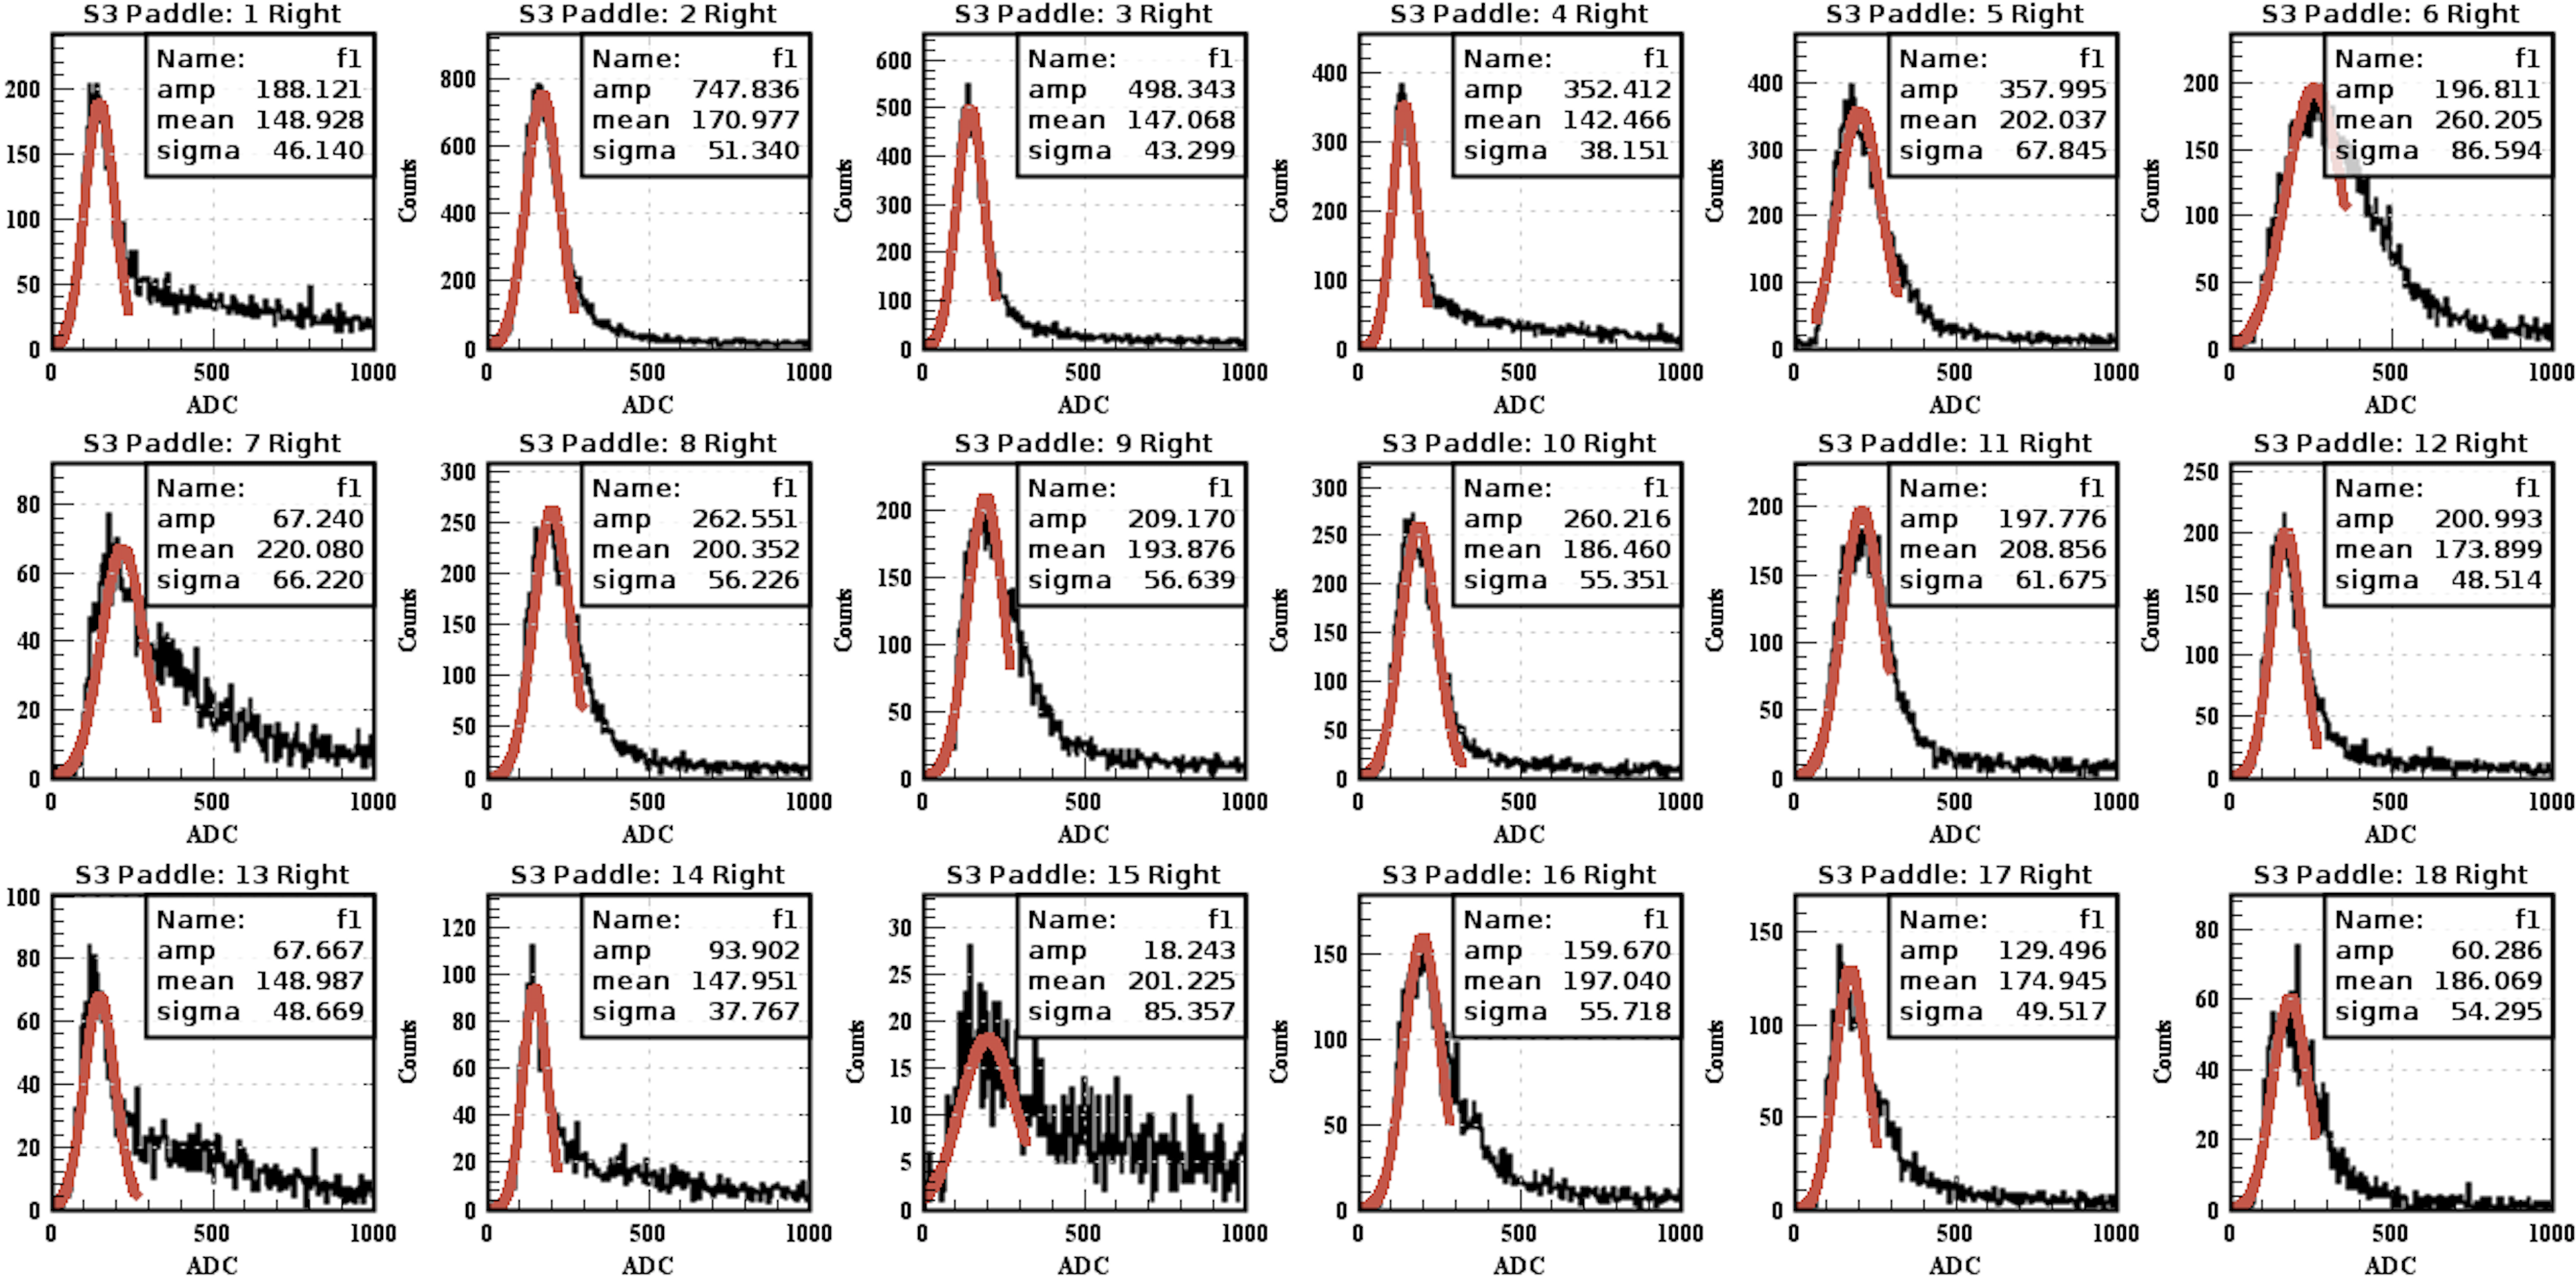
\includegraphics[width=0.95\columnwidth,keepaspectratio]{img/spe.png}
	\caption{The electronic scheme of the LTCC.}
	\label{fig:speCalibration}
\end{figure}


\paragraph{PMT gain matching}


\begin{figure}
	\centering
	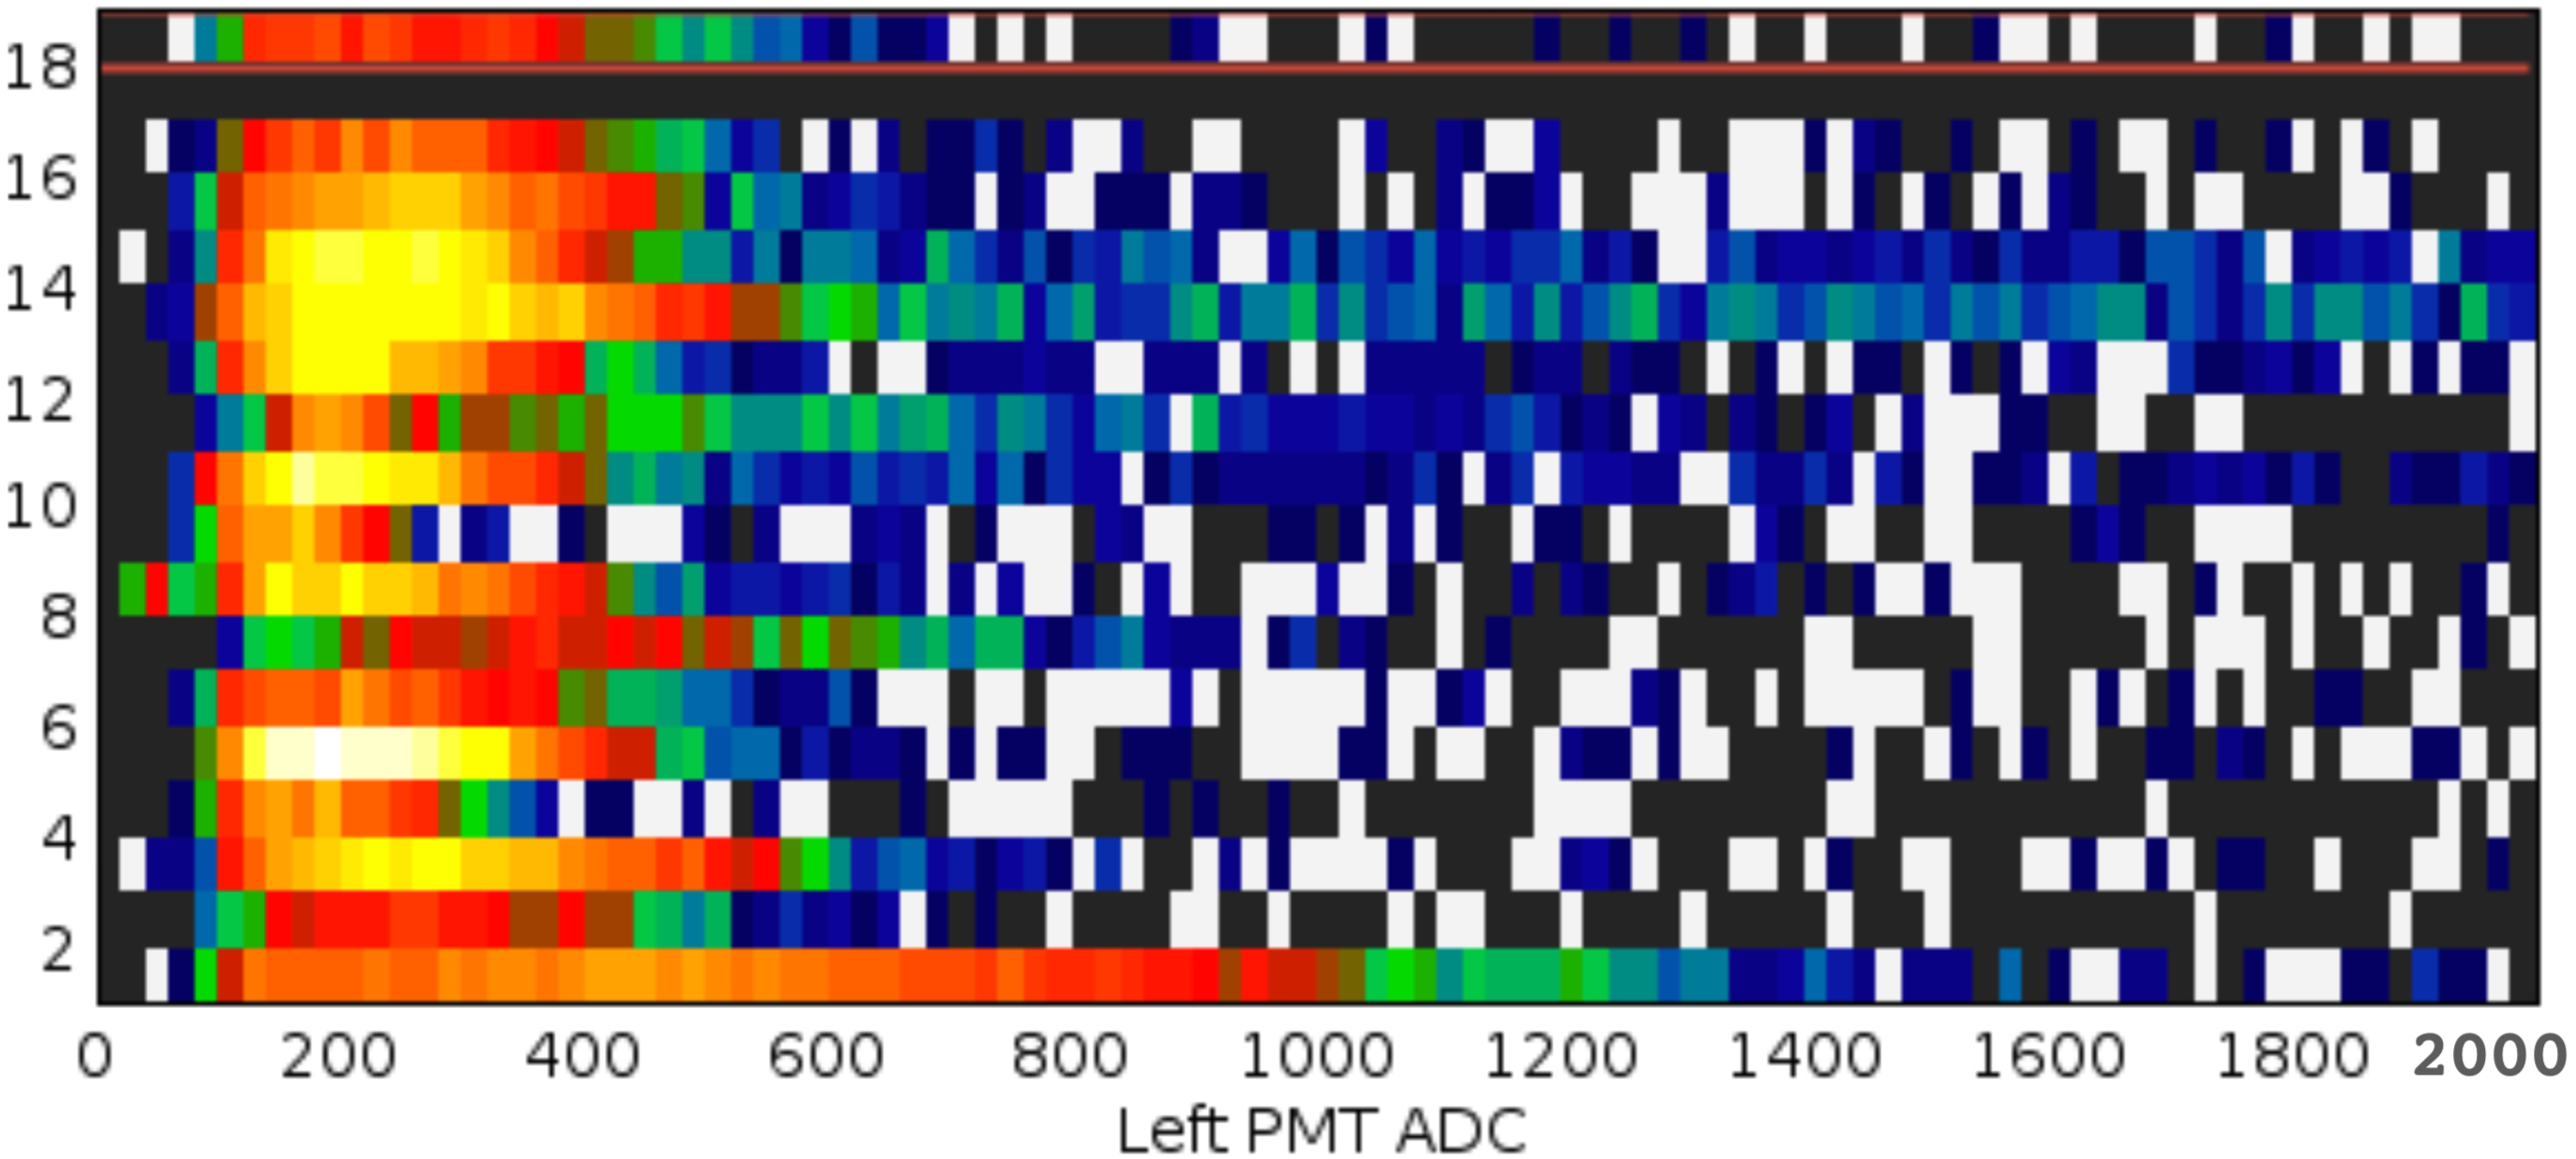
\includegraphics[width=0.95\columnwidth,keepaspectratio]{img/gainMatchingBefore.png}
	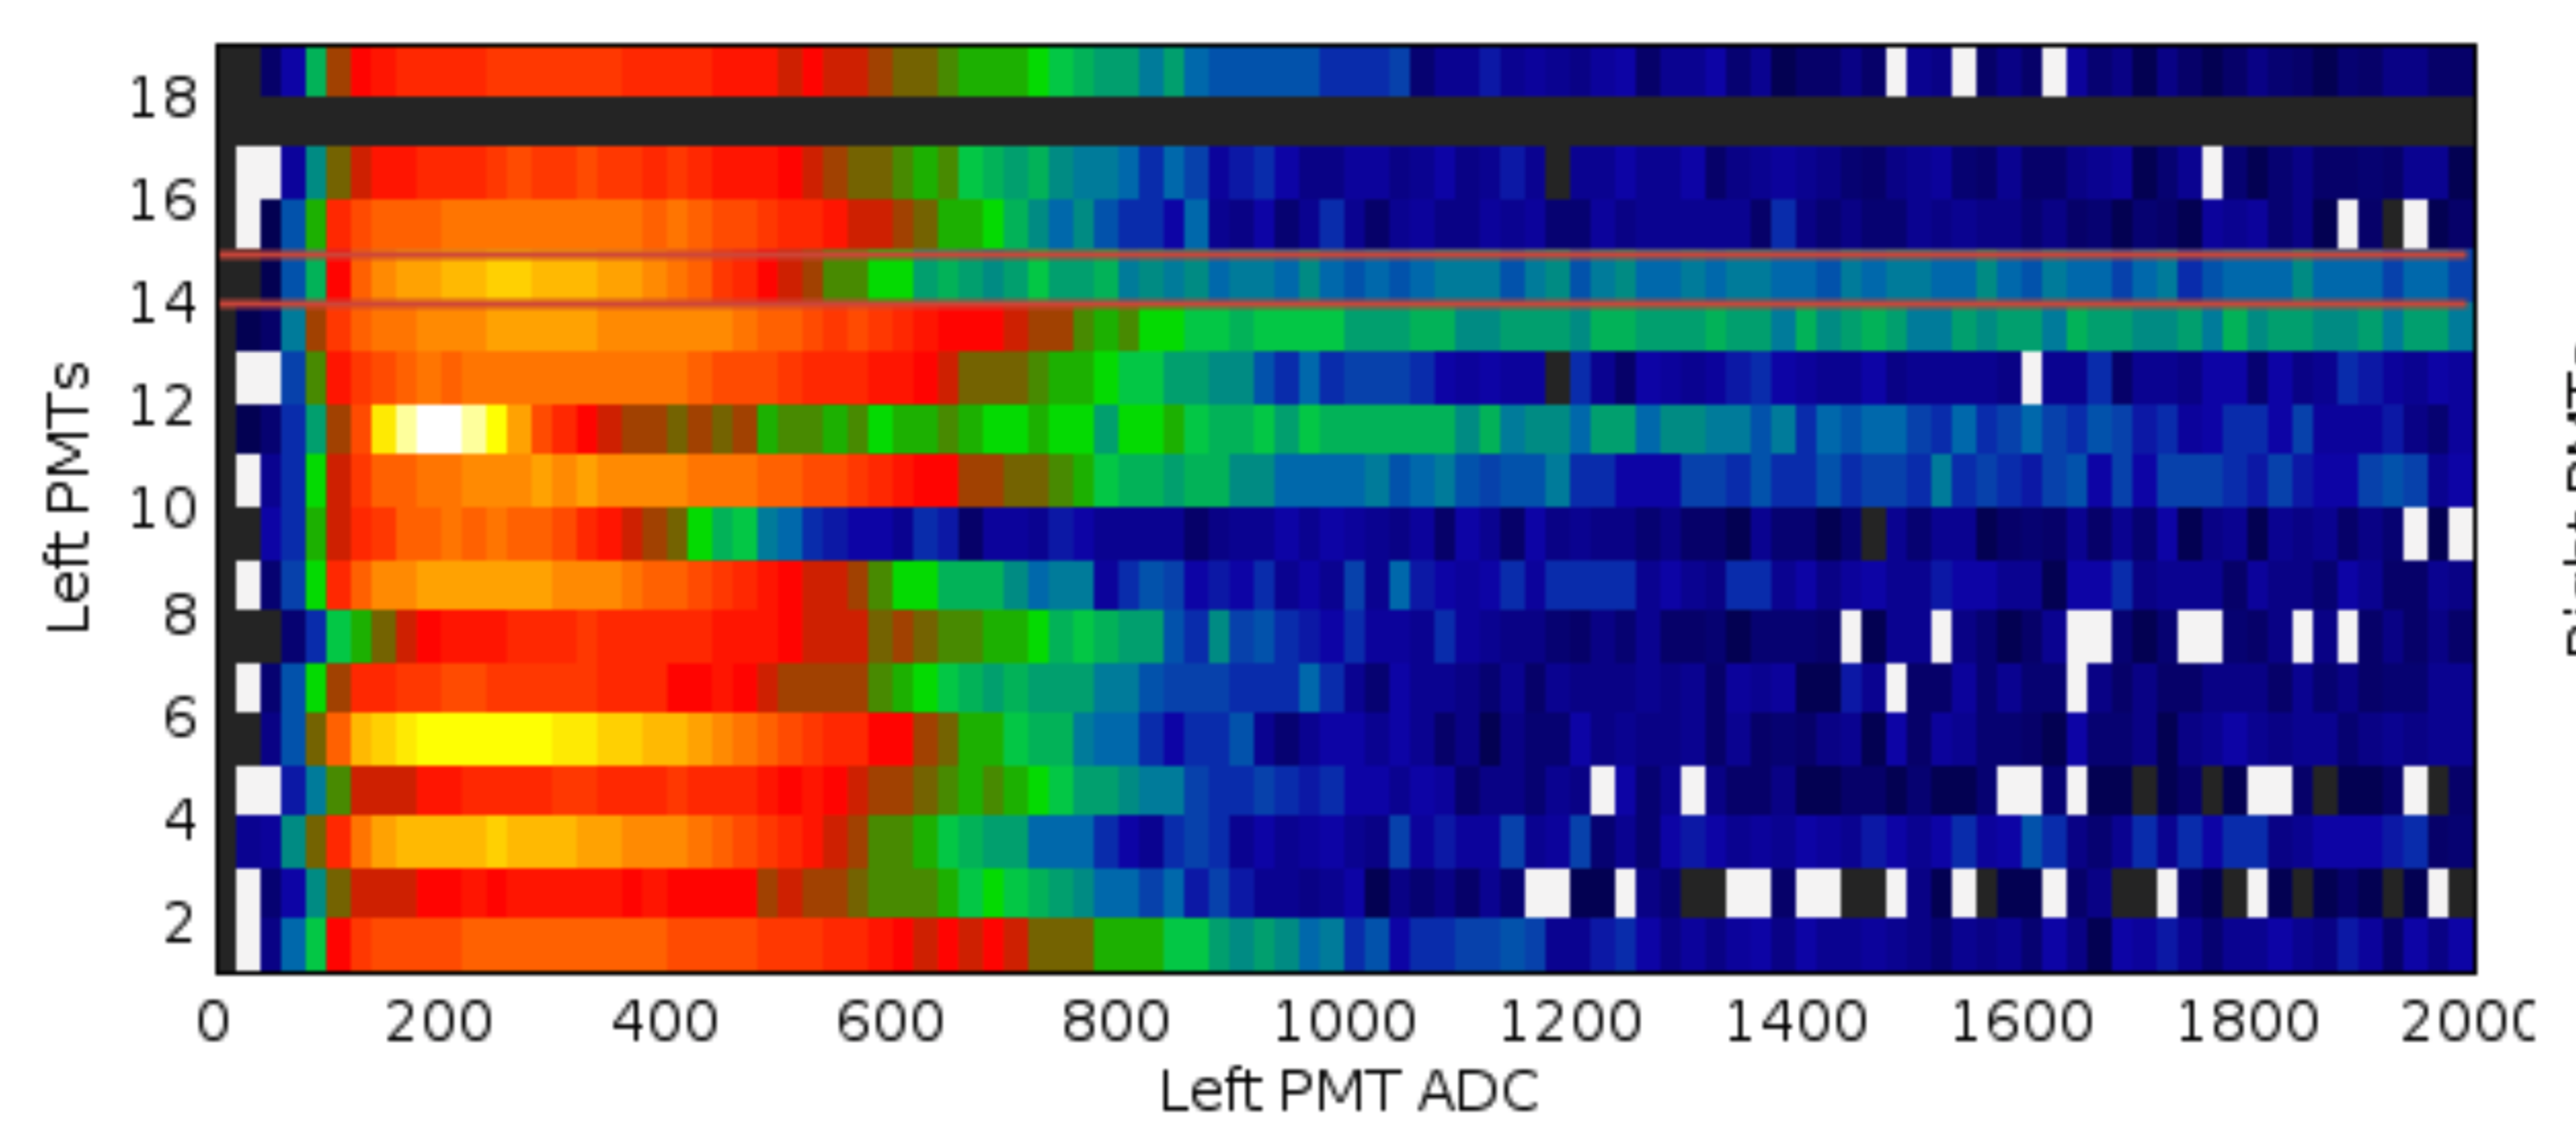
\includegraphics[width=0.95\columnwidth,keepaspectratio]{img/gainMatchingAfter.png}
	\caption{The electronic scheme of the LTCC.}
	\label{fig:gainMatching}
\end{figure}




